% manuscript.tex - minimal reproducible manuscript (fill figures/results folder)
\documentclass[11pt]{article}
\usepackage[utf8]{inputenc}
\usepackage{graphicx}
\usepackage{caption}
\usepackage{subcaption}
\usepackage{booktabs}
\usepackage{hyperref}
\usepackage{geometry}
\geometry{margin=1in}

\title{A reproducible machine learning survival pipeline identifies prognostic gene signatures in ovarian carcinoma}
\author{Diksha Singra\\Independent Researcher; M.Sc. Biotechnology\\\texttt{dikshasingra99@gmail.com}}
\date{}

\begin{document}
\maketitle

\begin{abstract}
We present a reproducible machine learning survival pipeline applied to ovarian carcinoma. The code, environment file, processed data and result figures are available in the project repository (\texttt{https://github.com/dikshasingra/TCGA\_OV\_PROJECT}). Key findings include an RSF model (C-index $\approx$0.60) and a small set of prognostic genes validated with Cox regression and Kaplan--Meier analysis.
\end{abstract}

\section{Introduction}
(Short intro — replace with your paragraphs about ovarian cancer, prognostic biomarkers, and motivation.)

\section{Materials and Methods}
Pipeline and environment are available in the repository. Briefly: processed gene expression + survival table were used; Random Survival Forest (RSF) for variable selection; Cox proportional hazards for multivariable testing; Kaplan--Meier and log-rank for group survival comparisons. See \texttt{methods.txt} for full reproducible commands.

\section{Results}
\subsection{Model performance}
Point estimates: RSF C-index $\approx$0.60; Cox C-index $\approx$0.63 (see \texttt{results/}).

\subsection{Top prognostic genes}
Top genes and KM figures saved in \texttt{figures/} and summary CSVs in \texttt{results/}. Example publication-ready KM plot: \texttt{figures/km\_GENE291\_GENE437\_pub.png}.

\begin{figure}[ht]
  \centering
  \begin{subfigure}{0.48\textwidth}
    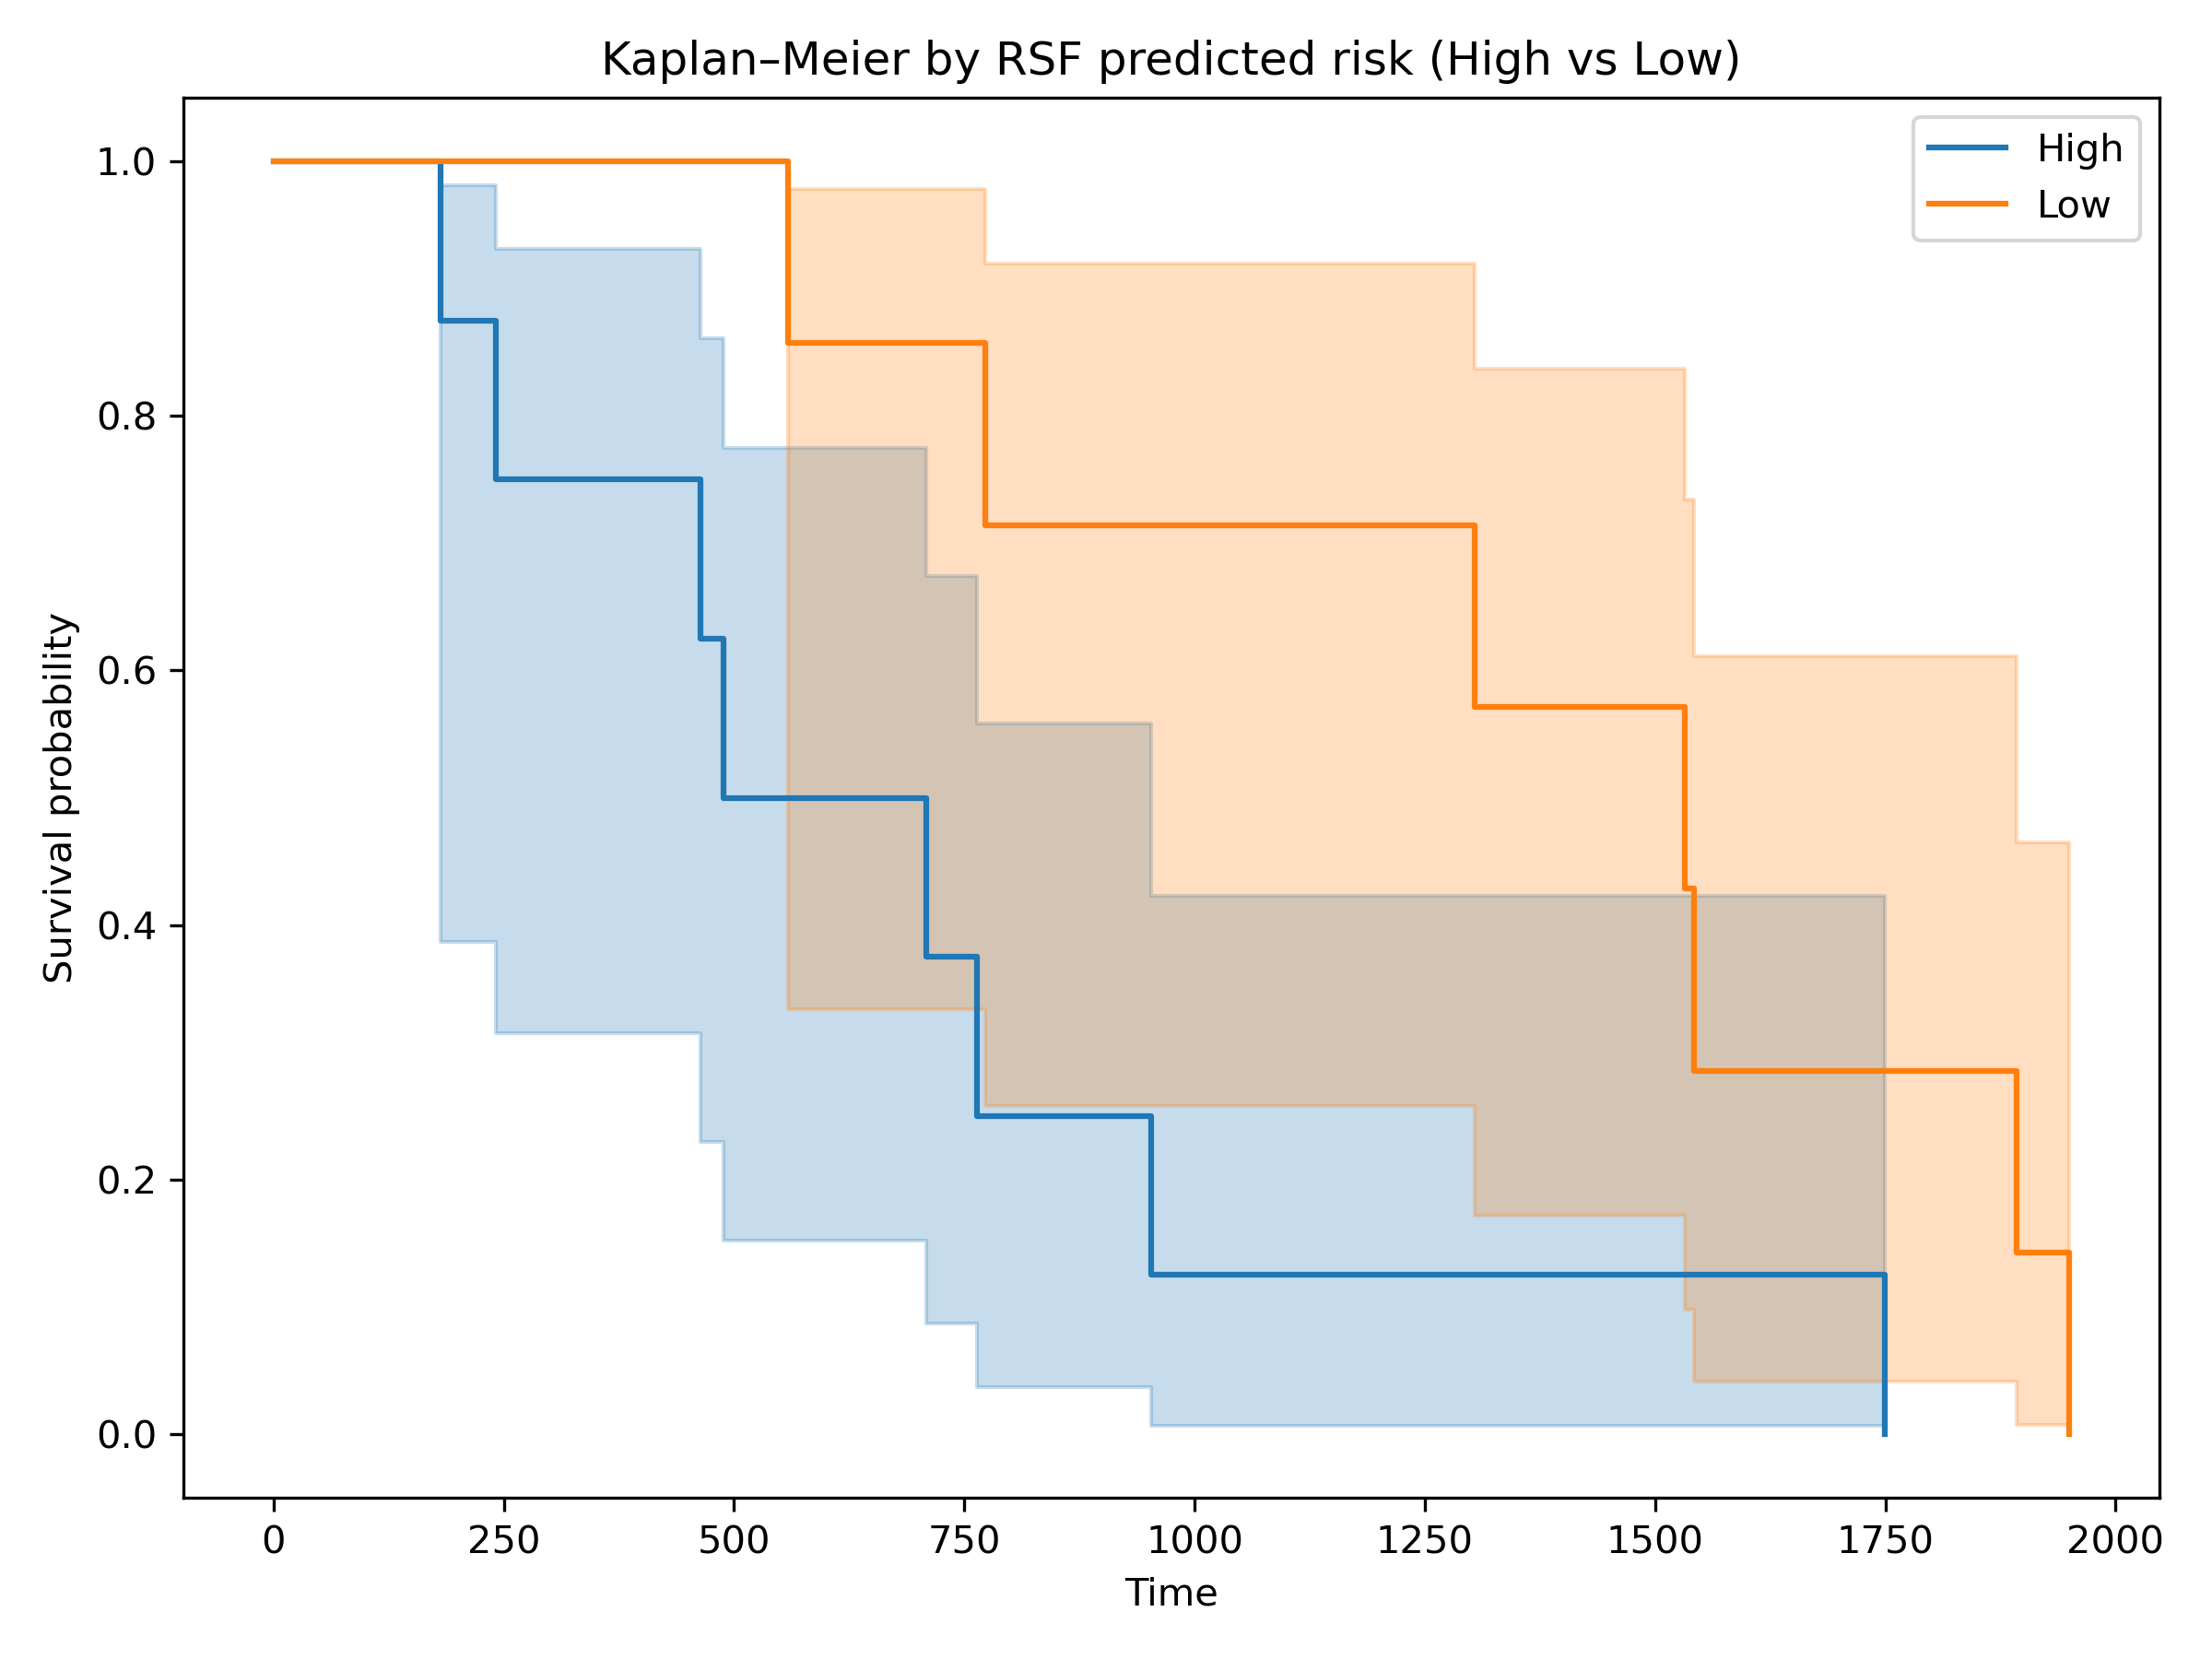
\includegraphics[width=\linewidth]{figures/km_plot.png}
    \caption{KM by predicted risk}
  \end{subfigure}\quad
  \begin{subfigure}{0.48\textwidth}
    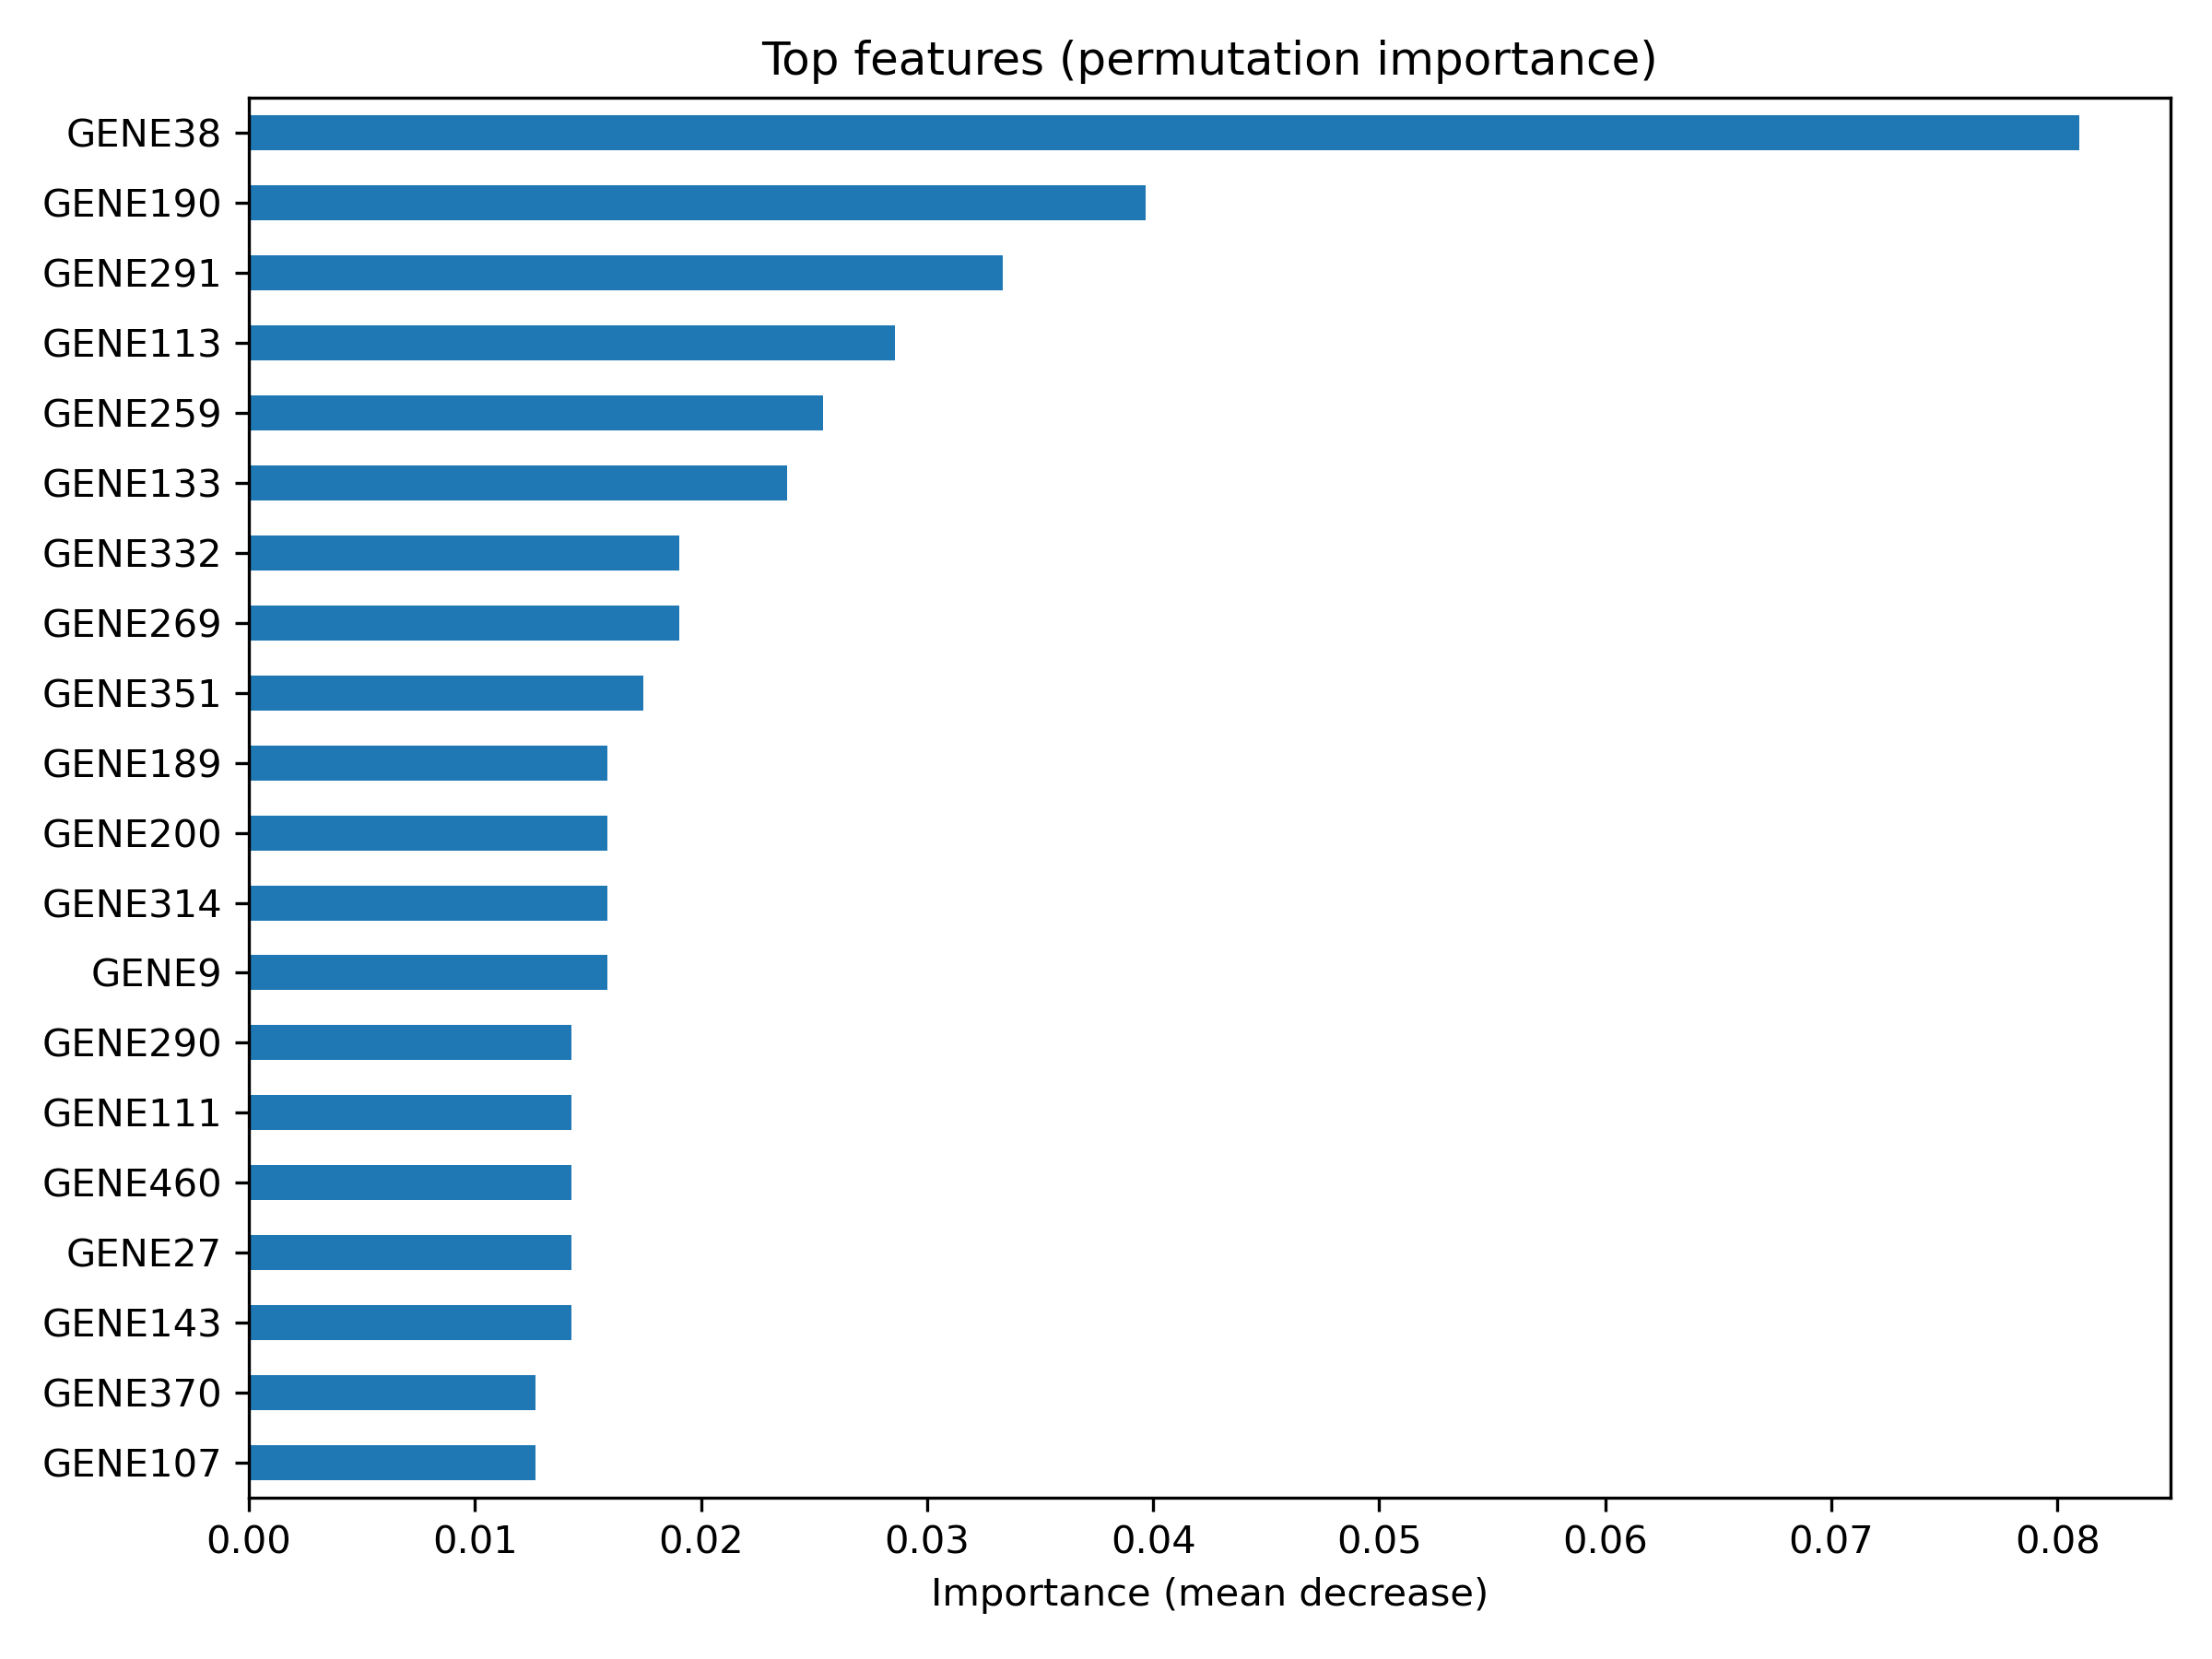
\includegraphics[width=\linewidth]{figures/feature_importance.png}
    \caption{Top feature importance}
  \end{subfigure}
  \caption{Representative results. Replace/adjust figures as needed.}
\end{figure}

\section{Discussion}
(Short discussion — explain biological relevance, limitations, and future work.)

\section{Reproducibility and Data}
All code, notebooks, conda environment and results are in the GitHub repository: \url{https://github.com/dikshasingra/TCGA_OV_PROJECT}. Raw + processed files are under \texttt{data\_raw/} and \texttt{data\_processed/}. See \texttt{README.md}.

\section{Acknowledgements}
Independent researcher project.

\bibliographystyle{plain}
\bibliography{references}

\end{document}